\chapter{Recurrent Neural Networks (RNN) \& RNNLM}


\begin{figure}[H]
    \centering
    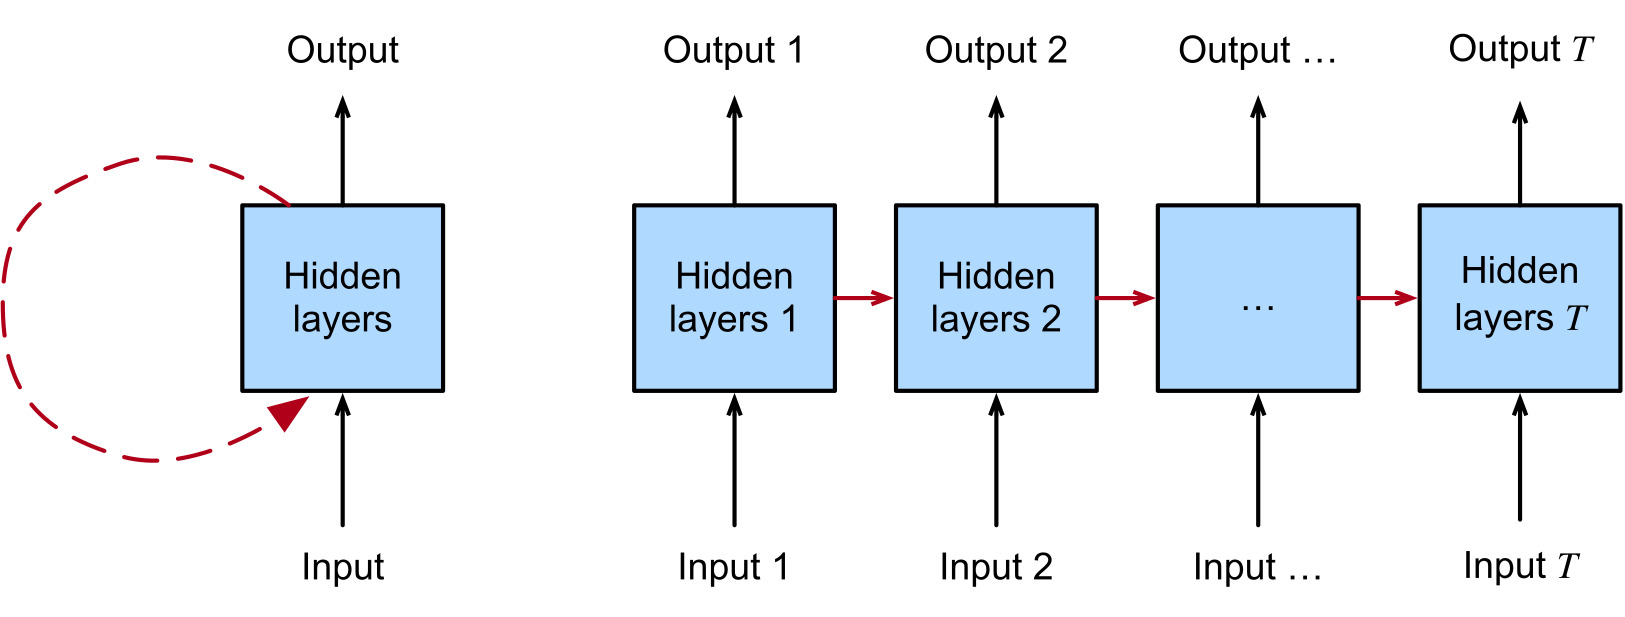
\includegraphics[width=\linewidth, height=3cm, keepaspectratio]{Pictures/Recurrent-Neural-Networks/unfolded-rnn.jpg}
    \caption*{On the left recurrent connections are depicted via cyclic edges. On the right, we unfold the RNN over time steps.}
\end{figure}


\begin{enumerate}
    \item A great many learning tasks require dealing with \textbf{sequential data}. 
    
    \item Image captioning, speech synthesis, and music generation all require that models produce outputs consisting of sequences. 
    
    \item In other domains, such as time series prediction, video analysis, and musical information retrieval, a model must learn from inputs that are sequences. 
    
    \item These demands often arise simultaneously: tasks such as translating passages of text from one natural language to another, engaging in dialogue, or controlling a robot, demand that models both ingest and output sequentially structured data.

    \item Recurrent neural networks (RNNs) are deep learning models that capture the dynamics of sequences via \textbf{recurrent connections}, which can be thought of as \textbf{cycles in the network of nodes}.

    \item It is the feedforward nature of neural networks that makes the order of computation unambiguous. \\
    However, recurrent edges are defined in a precise way that ensures that no such ambiguity can arise.

    \item Recurrent neural networks are \textbf{unrolled} across time steps (or sequence steps), with the same underlying parameters applied at each step. 
    
    \item While the standard connections are applied \textbf{synchronously} to propagate each layer’s activations to the subsequent layer at the same time step, the recurrent connections are \textbf{dynamic}, passing information across adjacent time steps.

    \item RNNs can be thought of as feedforward neural networks where each layer’s parameters (both conventional and recurrent) are shared across time steps.

    \item While the inputs and targets for many fundamental tasks in machine learning cannot easily be represented as fixed-length vectors, they can often nevertheless be represented as varying-length sequences of fixed-length vectors.\\
    \textbf{For example}: documents can be represented as sequences of words; medical records can often be represented as sequences of events (encounters, medications, procedures, lab tests, diagnoses); videos can be represented as varying-length sequences of still images.

    \item 
\end{enumerate}


\section{Working with Sequences \cite{dnn-1}}

\begin{customTableWrapper}{1.5}
\begin{longtable}{l l p{8cm}}
    $\mathbf{x}$ & $\in \mathbb{R}^d$ & single feature vector \\
    $\mathbf{x}_1, \cdots, \mathbf{x}_T$ & $\in \mathbb{R}^d$ & ordered list of feature vectors \\
    $\mathbf{x}_t$ & $\in \mathbb{R}^d$ & each feature vector \\
    $t$ & $\in \mathbb{Z}^+$ & time step \\
\end{longtable}
\end{customTableWrapper}


\begin{enumerate}[itemsep=0.15cm]
    \item Some datasets consist of a single \textbf{massive sequence}\\
    \textbf{For example}, the extremely long streams of sensor readings that might be available to climate scientists.\\
    In such cases, we might create training datasets by randomly sampling subsequences of some predetermined length.

    \item Often data arrives as a \textbf{collection of sequences}\\
    \textbf{Examples}:
    \begin{enumerate}
        \item a collection of documents, each represented as its own sequence of words, and each having its own length $T_i$
        
        \item sequence representation of patient stays in the hospital, where each stay consists of a number of events and the sequence length depends roughly on the length of the stay.
        
    \end{enumerate}

    \item we \textbf{CANNOT} assume that the data arriving at each time step are independent of each other.\\
    \textbf{For example}, the words that likely to appear later in a document depend heavily on words occurring earlier in the document.\\
    The medicine a patient is likely to receive on the 10th day of a hospital visit depends heavily on what transpired in the previous nine days.

    \item we require only that the sequences themselves are sampled from some fixed underlying distribution over entire sequences

    \item sequence-to-sequence tasks take two forms: 
    \begin{enumerate}
        \item \textbf{aligned}: where the input at each time step aligns with a corresponding target (e.g., part of speech tagging); 
        
        \item \textbf{unaligned}: where the input and target do not necessarily exhibit a step-for-step correspondence (e.g., machine translation).
    \end{enumerate}

    \item we can tackle the most straightforward problem: unsupervised density modeling (also called sequence modeling). Here, given a collection of sequences, our goal is to estimate the probability mass function that tells us how likely we are to see any given sequence, i.e., $p(\mathbf{x}_1, \ldots, \mathbf{x}_T)$

\end{enumerate}


\section{Autoregressive Models \cite{dnn-1}} \label{Autoregressive Models}

\begin{customTableWrapper}{1.5}
\begin{table}[H]
    \centering
    \begin{tabular}{l p{8cm}}
        $P(x_t \mid x_{t-1}, \ldots, x_1)$ & probability distribution \\
        $\mathbb{E}[(x_t \mid x_{t-1}, \ldots, x_1)]$ & conditional expectation \\
    \end{tabular}
\end{table}
\end{customTableWrapper}

\begin{enumerate}
    \item At each time step $t$, we observe the input, $x_t$, of the index at that time.

    \item models that regress the value of a signal on the previous values of that same signal are naturally called \textbf{autoregressive models}.

    \item There is just one major problem: the number of inputs, $x_{t-1}, \cdots, x_1$ varies, depending on $t$.\\
    In other words, the number of inputs increases with the amount of data that we encounter. \\
    Thus if we want to treat our historical data as a training set, we are left with the problem that each example has a different number of features.

    \item we might believe that although long sequences $x_{t-1}, \ldots, x_1$ are available, it may not be necessary to look back so far in the history when predicting the near future.\\
    In this case we might content ourselves to condition on some window of length $\tau$ and only use $x_{t-1}, \ldots, x_{t-\tau}$ observations.\\
    The immediate benefit is that now the number of arguments is always the same, at least for $t > \tau$.\\
    This allows us to train any linear model or deep network that requires fixed-length vectors as inputs.

    \item we might develop models that maintain some summary $h_t$ of the past observations and at the same time update $h_t$ in addition to the prediction $\hat{x}_t$.\\
    This leads to models that estimate not only $x_t$ with $\hat{x}_t = P(x_t \mid h_{t})$ but also updates of the form $h_t = g(h_{t-1}, x_{t-1})$. \\
    Since $h_t$ is never observed, these models are also called \textbf{latent autoregressive models}\indexlabel{latent autoregressive models}.

    \item To construct training data from historical data, one typically creates examples by sampling windows randomly.

    \item we often assume that while the specific values of $x_t$ might change, the dynamics according to which each subsequent observation is generated given the previous observations do not. Statisticians call dynamics that do not change \textbf{stationary}.
    
\end{enumerate}




\section{Sequence Models \cite{dnn-1}} \label{Sequence Models}

\begin{enumerate}
    \item especially when working with language, we wish to estimate the joint probability of an entire sequence\\
    Generally, these estimated functions are called sequence models and for natural language data, they are called language models.

    \item The field of sequence modeling has been driven so much by natural language processing, that we often describe sequence models as “language models”, even when dealing with non-language data.

    \item language modeling gives us not only the capacity to evaluate likelihood, but the ability to sample sequences, and even to optimize for the most likely sequences.

    \item While language modeling might not, at first glance, look like an autoregressive problem, we can reduce language modeling to autoregressive prediction by decomposing the joint density of a sequence $p(x_1, \ldots, x_T)$ into the product of conditional densities in a left-to-right fashion by applying the chain rule of probability:
    \[
        \hfill
        P(x_1, \cdots, x_T) = P(x_1) \dprod_{t=2}^T P(x_t \mid x_{t-1}, \cdots, x_1)
        \hfill
    \]

    \item If we are working with discrete signals such as words, then the autoregressive model must be a probabilistic classifier, outputting a full probability distribution over the vocabulary for whatever word will come next, given the leftwards context.

\end{enumerate}


\section{Markov Models \cite{dnn-1}}\label{rnn: Markov Models}

\begin{enumerate}
    \item we condition only on the $\tau$ previous time steps, i.e., $x_{t-1}, \ldots, x_{t-\tau}$, rather than the entire sequence history $x_{t-1}, \ldots, x_1$.
    
    \item Whenever we can throw away the history beyond the previous $\tau$ steps without any loss in predictive power, we say that the sequence satisfies a \textbf{Markov condition}\indexlabel{Markov condition}, i.e., that \textit{the future is conditionally independent of the past, given the recent history}. 
    
    \item When $\tau = 1$, we say that the data is characterized by a \textbf{first-order Markov model}\indexlabel{first-order Markov model}, and when $\tau = k$, we say that the data is characterized by a $k^{\textrm{th}}$-order Markov model.
    
    \item For when the first-order Markov condition holds ($\tau = 1$) the factorization of our joint probability becomes a product of probabilities of each word given the previous word:
    \[
        \hfill
        P(x_1, \ldots, x_T) = P(x_1) \prod_{t=2}^T P(x_t \mid x_{t-1})
        \hfill
    \]

    \item we compromise, obviating computational and statistical difficulties by training models whose validity depends on a $k^{\textrm{th}}$-order Markov condition.

    \item With discrete data, a true Markov model simply counts the number of times that each word has occurred in each context, producing the relative frequency estimate of $P(x_t \mid x_{t-1})$.\\
    Whenever the data assumes only discrete values (as in language), the most likely sequence of words can be computed efficiently using \textbf{dynamic programming}.

\end{enumerate}

\subsection{Order of Decoding \cite{dnn-1}}

\begin{enumerate}[itemsep=0.15cm]
    \item the factorization of a text sequence $P(x_1, \ldots, x_T)$ as a \textbf{left-to-right} chain of conditional probabilities and not right-to-left or some other, seemingly random order.
    \[
        \hfill
        P(x_1, \ldots, x_T) = P(x_T) \prod_{t=T-1}^1 P(x_t \mid x_{t+1}, \ldots, x_T)
        \hfill
    \]

    \item there is nothing wrong with unfolding in reverse order.\\
    However, there are many reasons why factorizing text in the same direction in which we read it (left-to-right for most languages, but right-to-left for Arabic and Hebrew) is preferred for the task of language modeling.

    \item this is just a more natural direction for us to think about\\
    ability to anticipate which words and phrases are likely to come next\\
    even if we had no other reason to prefer such in-order decodings, they would be useful if only because we have better intuitions for what should be likely when predicting in this order.

    \item by factorizing in order, we can assign probabilities to arbitrarily long sequences using the same language model.\\
    To convert a probability over steps $1$ through $t$ into one that extends to word $t+1$ we simply multiply by the conditional probability of the additional token given the previous ones: 
    \[
        \hfill
        P(x_{t+1}, \ldots, x_1) = P(x_{t}, \ldots, x_1) \cdot P(x_{t+1} \mid x_{t}, \ldots, x_1)
        \hfill
    \]

    \item we have stronger predictive models for predicting adjacent words than words at arbitrary other locations. \\
    While all orders of factorization are valid, they do not necessarily all represent equally easy predictive modeling problems.\\
    we believe that future events cannot influence the past. Hence, if we change $x_t$, we may be able to influence what happens for $x_{t+1}$ going forward but not the converse.\\
    That is, if we change $x_t$, the distribution over past events will not change.\\
    In some contexts, this makes it easier to predict $P(x_{t+1} \mid x_t)$ than to predict $P(x_t \mid x_{t+1})$\\
    we can find $x_{t+1} = f(x_t) + \epsilon$ for some additive noise $\epsilon$, whereas the converse is not true

    
\end{enumerate}




\section{Language Models \cite{dnn-1}} \label{Language Models}

SEE: \fullref{Sequence Models}

\begin{enumerate}
    \item Assume that the tokens in a text sequence of length $T$ are in turn $x_1, x_2, \cdots, x_T$

    \item The goal of language models is to estimate the joint probability of the whole sequence: $P(x_1, x_2, \ldots, x_T)$ 

    \item an ideal language model should generate natural text on its own, simply by drawing one token at a time $x_t \sim P(x_t \mid x_{t-1}, \ldots, x_1)$

    \item Quite unlike the monkey using a typewriter, all text emerging from such a model would pass as natural language, e.g., English text

    \item it would be sufficient for generating a meaningful dialog, simply by conditioning the text on previous dialog fragments.

    
\end{enumerate}


\subsection{Converting Raw Text into Sequence Data \cite{dnn-1}}

\begin{enumerate}
    \item we will need some basic tools for converting raw text into sequences of the appropriate form.

    \item Typical preprocessing pipelines execute the following steps:
    \begin{enumerate}
        \item Load text as strings into memory.

        \item Split the strings into tokens (e.g., words or characters).

        \item Build a vocabulary dictionary to associate each vocabulary element with a numerical index.

        \item Convert the text into sequences of numerical indices.

    \end{enumerate}
\end{enumerate}


\subsubsection{Tokenization \cite{dnn-1}}

\begin{enumerate}
    \item Tokens are the atomic (indivisible) units of text. Each time step corresponds to 1 token, but what precisely constitutes a token is a design choice. 
    
    \item \textbf{For example}, we could represent the sentence “Baby needs a new pair of shoes” as a sequence of 7 words, where the set of all words comprise a large vocabulary (typically tens or hundreds of thousands of words).\\
    Or we would represent the same sentence as a much longer sequence of 30 characters, using a much smaller vocabulary (there are only 256 distinct ASCII characters).

    \item These tokens are still strings.

\end{enumerate}

\subsubsection{Vocabulary \cite{dnn-1}}

\begin{enumerate}
    \item the inputs to our models must ultimately consist of numerical inputs

    \item we determine the set of \textbf{unique tokens} in our training corpus. 
    
    \item We then assign a \textbf{numerical index} to each unique token. 
    
    \item \textbf{Rare vocabulary elements} are often \textbf{dropped} for convenience. 
    
    \item Whenever we encounter a token at training or test time that had not been previously seen or was dropped from the vocabulary, we represent it by a special “\verb|<unk>|” token, signifying that this is an \textbf{unknown value}.

    \item Note that we have not lost any information and can easily convert our dataset back to its original (string) representation.

\end{enumerate}


\section{Partitioning Sequences \cite{dnn-1}} \label{Partitioning Sequences}

\begin{figure}[H]
    \centering
    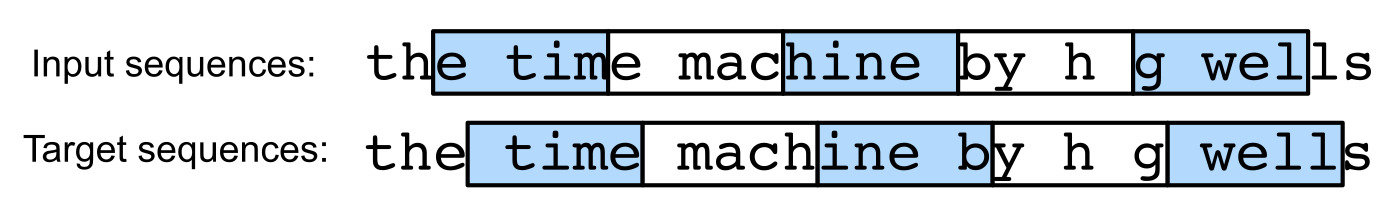
\includegraphics[width=\linewidth, height=1.5cm, keepaspectratio]{Pictures/Recurrent-Neural-Networks/Partitioning-Sequences.jpg}
    \caption*{Obtaining five pairs of input sequences and target sequences from partitioned length-5 subsequences. ($n=5$ and $d=2$)}
\end{figure}


\begin{customTableWrapper}{1.5}
\begin{table}[H]
    \centering
    \begin{tabular}{l p{8cm}}
        $T$ & length of sequence (num of tokens in corpus) \\
        $n$ & length of subsequence (num of tokens in input/ timesteps) \\
        $d\in [0,n)$ & randomness to discard the first few tokens \\
        $m$ & chunk size of remaining subsequence \\
    \end{tabular}
\end{table}
\end{customTableWrapper}


\begin{enumerate}
    \item Suppose that the dataset takes the form of a sequence of $T$ token indices in corpus. 
    
    \item We will partition it into subsequences, where each subsequence has $n$ tokens (time steps).

    \item To iterate over (almost) all the tokens of the entire dataset for each epoch and obtain all possible length-$n$ subsequences, we can introduce \textbf{randomness}.

    \item at the beginning of each epoch, discard the first $d$ tokens, where $d\in [0,n)$ is uniformly sampled at random.

    \item The rest of the sequence is then partitioned into $m=\lfloor (T-d)/n \rfloor$ subsequences.\\
    Denote by $\mathbf x_t = [x_t, \cdots, x_{t+n-1}]$ the length-$n$ subsequence starting from token $x_t$ at time step $t$.\\
    The resulting $m$ partitioned subsequences are $\mathbf x_d, \mathbf x_{d+n}, \cdots, \mathbf x_{d+n(m-1)}$.\\
    Each subsequence will be used as an input sequence into the language model.

\end{enumerate}








\section{Recurrent Neural Networks (RNN) \cite{dnn-1}} \label{Recurrent Neural Networks (RNN)}

\begin{customTableWrapper}{1.5}
\begin{table}[H]
    \centering
    \begin{tabular}{l p{8cm}}
        $x_t$ & token \\
        $t$ & time step \\
        $\mathcal{V}$ & vocabulary set \\
        
    \end{tabular}
\end{table}
\end{customTableWrapper}


\begin{enumerate}
    \item we described Markov models and $n$-grams for language modeling, where the conditional probability of token $x_t$ at time step $t$ only depends on the $n-1$ previous tokens.

    \item If we want to incorporate the possible effect of tokens earlier than time step $t - (n-1)$ on $x_t$, we need to increase $n$

    \item the number of model parameters would also increase exponentially with it, as we need to store $|\mathcal{V}|^n$ numbers for a vocabulary set $\mathcal{V}$.

    \item rather than modeling $P(x_t \mid x_{t-1}, \ldots, x_{t-n+1})$ it is preferable to use a latent variable model $P(x_t \mid x_{t-1}, \ldots, x_1) \approx P(x_t \mid h_{t-1})$, where $h_{t-1}$ is a hidden state that stores the sequence information up to time step $t-1$

    \item the hidden state at any time step $t$ could be computed based on both the current input $x_t$ and the previous hidden state $h_{t-1}$: $h_t = f(x_{t}, h_{t-1})$.

    \item For a sufficiently powerful function $f$, the latent variable model is not an approximation.\\
    After all, $h_t$ may simply store all the data it has observed so far.\\ 
    However, it could potentially make both computation and storage expensive.

    \item It is noteworthy that hidden layers and hidden states refer to two very different concepts.\\
    \textbf{Hidden layers} are layers that are hidden from view on the path from input to output.\\
    \textbf{Hidden states} are technically speaking inputs to whatever we do at a given step, and they can only be computed by looking at data at previous time steps.

    \item Recurrent neural networks (RNNs) are neural networks with hidden states.
\end{enumerate}


\subsection{Neural Networks without Hidden States \cite{dnn-1}}

\begin{customTableWrapper}{1.5}
\begin{longtable}{l l p{8cm}}
    \hline
    \customTableHeaderColor
    \multicolumn{3}{c}{\textbf{Input Layer}} \\ \hline
    $n$ & $\in \mathbb{R}$ & batch size \\
    $d$ & $\in \mathbb{R}$ & inputs \\
    $q$ & $\in \mathbb{R}$ & number of output classes \\
    $\mathbf{X}$ & $\in \mathbb{R}^{n \times d}$ & minibatch of examples \\

    \hline
    \customTableHeaderColor
    \multicolumn{3}{c}{\textbf{Hidden Layer}} \\ \hline
    $h$ & $\in \mathbb{R}$ & number of hidden units\\
    $\mathbf{W}_{\textrm{xh}}$ & $\in \mathbb{R}^{d \times h}$ & weight parameter \\
    $\mathbf{b}_\textrm{h}$ & $\in \mathbb{R}^{1 \times h}$ & bias parameter \\
    $\phi$ & & hidden layer’s activation function \\
    $\mathbf{H} = \phi(\mathbf{X} \mathbf{W}_{\textrm{xh}} + \mathbf{b}_\textrm{h})$ & $\in \mathbb{R}^{n \times h}$ & hidden layer output \\

    \hline
    \customTableHeaderColor
    \multicolumn{3}{c}{\textbf{Output Layer}} \\ \hline
    $\mathbf{W}_{\textrm{hq}}$ & $\in \mathbb{R}^{h \times q}$ &  weight parameter \\
    $\mathbf{b}_\textrm{q}$ & $\in \mathbb{R}^{1 \times q}$ & bias parameter \\
    $\mathbf{O} = \mathbf{H} \mathbf{W}_{\textrm{hq}} + \mathbf{b}_\textrm{q}$ & $\in \mathbb{R}^{n \times q}$ & output variable \\
    $\mathrm{softmax}(\mathbf{O})$ & $\in \mathbb{R}^{1 \times q}$ &  \\
\end{longtable}
\end{customTableWrapper}


\subsection{Recurrent Neural Networks with Hidden States \cite{dnn-1}}

\begin{figure}[H]
    \centering
    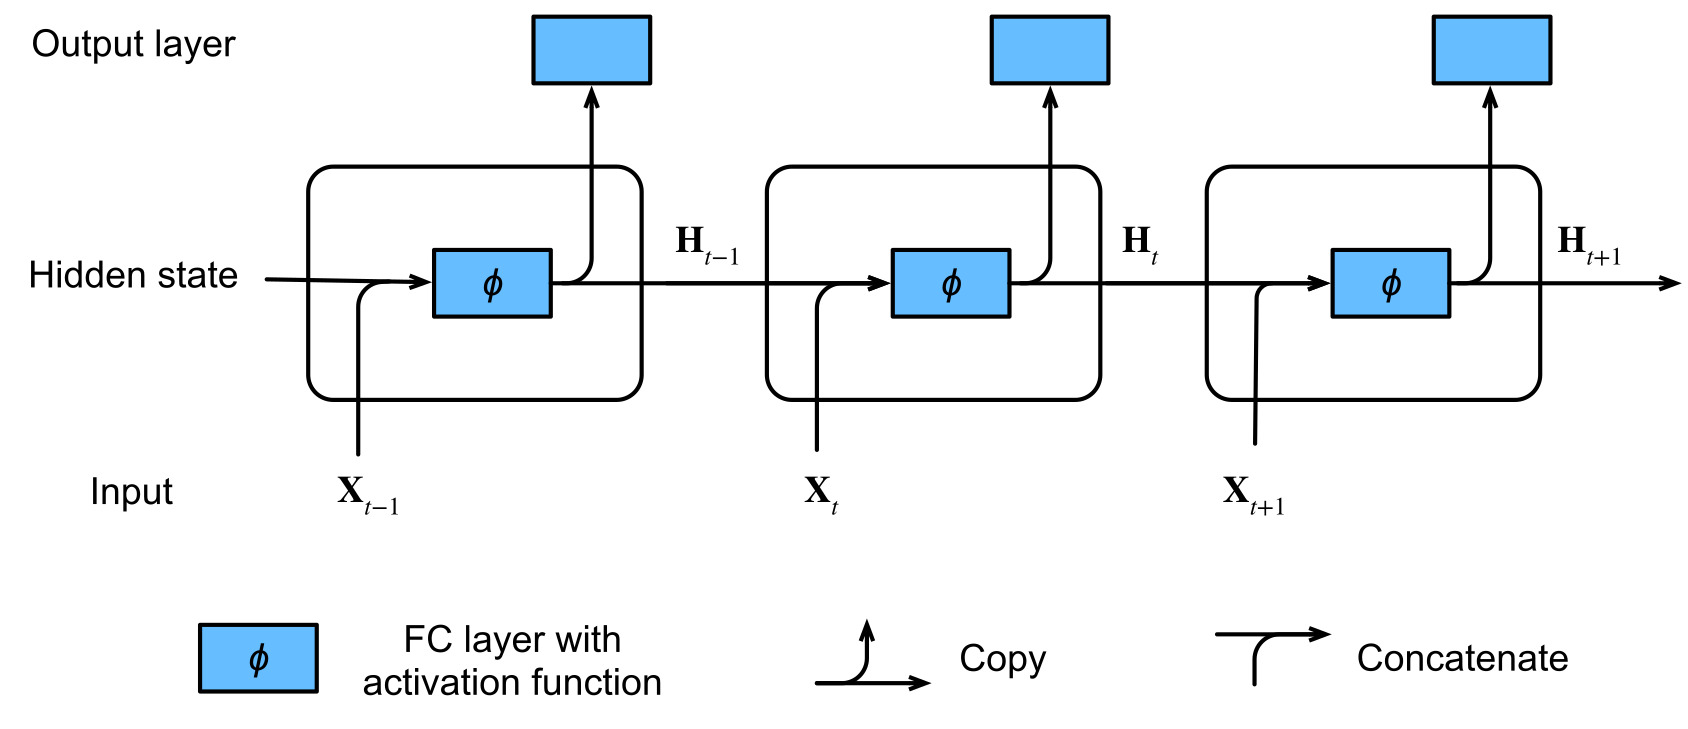
\includegraphics[width=\linewidth, height=3cm, keepaspectratio]{Pictures/Recurrent-Neural-Networks/rnn.jpg}
\end{figure}

\begin{customTableWrapper}{1.5}
        \begin{longtable}{l l p{4cm}}
            $t$ & $\in \mathbb{R}$ & time step \\
            
            $n$ & $\in \mathbb{R}$ & number of sequence examples \\
            
            $\mathbf{X}_t$ & $\in \mathbb{R}^{n \times d}$ & minibatch of inputs at time step $t$ \\
        
            \hline
            
            $\mathbf{H}_t$ & $\in \mathbb{R}^{n \times h}$ & hidden layer output of time step $t$ \\
            
            $\mathbf{H}_{t-1}$ & $\in \mathbb{R}^{n \times h}$ & hidden layer output from the previous time step \\
            
            $\mathbf{W}_{\textrm{hh}}$ & $\in \mathbb{R}^{h \times h}$ & weight parameter to describe how to use the hidden layer output of the previous time step in the current time step \\
        
            \hline
        
            $\mathbf{W}_{\textrm{hq}}$ & $\in \mathbb{R}^{h \times q}$ & weights \\
        
            $\mathbf{b}_\textrm{q}$ & $\in \mathbb{R}^{1 \times q}$ & bias \\
        
            $\mathbf{O}_t = \mathbf{H}_t \mathbf{W}_{\textrm{hq}} + \mathbf{b}_\textrm{q}$ & $\in \mathbb{R}^{1 \times q}$ & output of the output layer for time step $t$\\
        
            
        \end{longtable}
        \end{customTableWrapper}

\begin{enumerate}
    \item the calculation of the hidden layer output of the current time step is determined by the input of the current time step together with the hidden layer output of the previous time step:
    \[
        \hfill
        \mathbf{H}_t = \phi(\mathbf{X}_t \mathbf{W}_{\textrm{xh}} + \mathbf{H}_{t-1} \mathbf{W}_{\textrm{hh}}  + \mathbf{b}_\textrm{h})
        \hfill
    \]

    \item From the relationship between hidden layer outputs $\mathbf{H}_t$ and $\mathbf{H}_{t-1}$ of adjacent time steps, we know that these variables captured and retained the sequence’s historical information up to their current time step, just like the state or memory of the neural network’s current time step.

    \item Therefore, such a hidden layer output is called a \textbf{hidden state}. 
            
    \item Since the hidden state uses the same definition of the previous time step in the current time step, the computation is \textbf{recurrent}. 
    
    \item Hence, neural networks with hidden states based on recurrent computation are named \textbf{recurrent neural networks}. 
    
    \item Layers that perform the computation of (9.4.5) in RNNs are called \textbf{recurrent layers}.

    \item At any time step $t$, the computation of the hidden state can be treated as: 
    \begin{enumerate}
        \item concatenating the input $\mathbf{X}_t$ at the current time step $t$ and the hidden state $\mathbf{H}_{t-1}$ at the previous time step $t-1$

        \item feeding the concatenation result into a fully connected layer with the activation function $\phi$.
        
        \item The output of such a fully connected layer is the hidden state $\mathbf{H}_t$ of the current time step $t$. 
        
        \item In this case, the model parameters are the concatenation of $\mathbf{W}_{\textrm{xh}}$ and $\mathbf{W}_{\textrm{hh}}$, and a bias of $\mathbf{b}_\textrm{h}$.

        \item The hidden state of the current time step $t$, $\mathbf{H}_t$, will participate in computing the hidden state $\mathbf{H}_{t+1}$ of the next time step $t+1$.
        
        \item What is more, $\mathbf{H}_t$ will also be fed into the fully connected output layer to compute the output $\mathbf{O}_t$ of the current time step $t$.
    \end{enumerate}
\end{enumerate}


\section{RNN-Based Character-Level Language Models \cite{dnn-1}}

\begin{figure}[H]
    \centering
    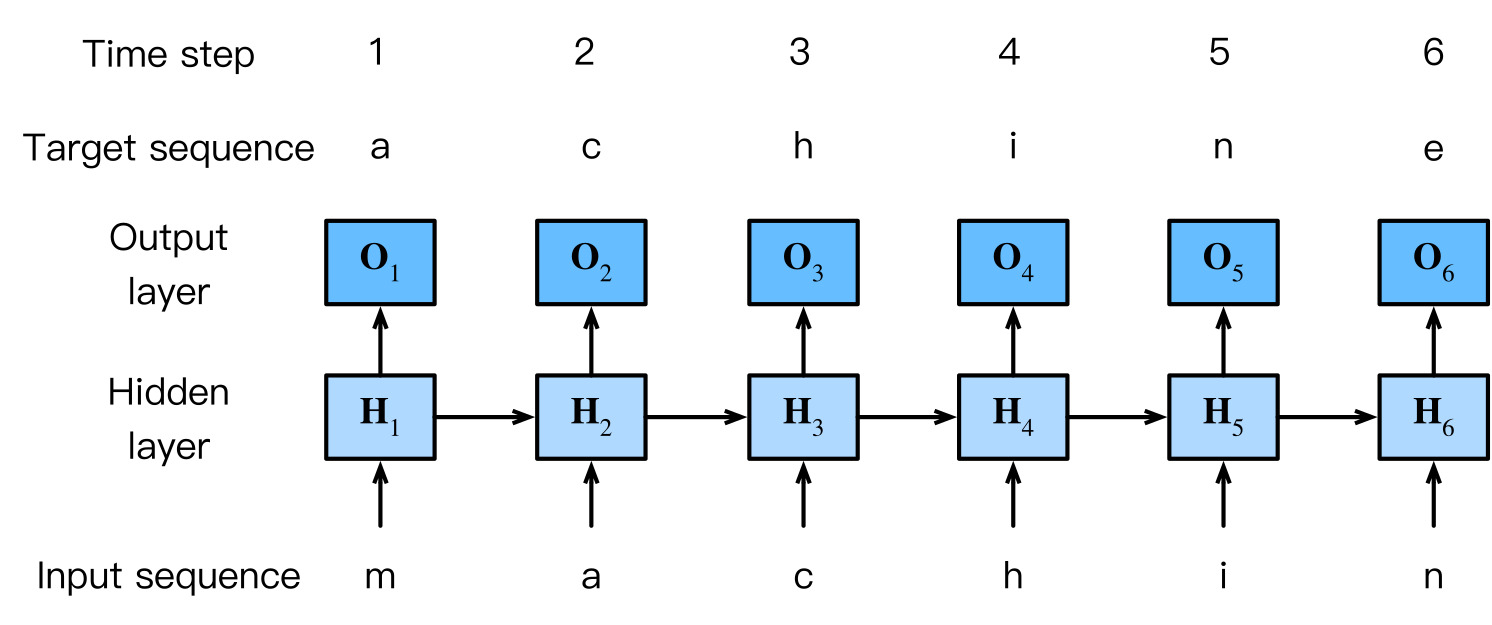
\includegraphics[width=\linewidth, height=4cm, keepaspectratio]{Pictures/Recurrent-Neural-Networks/rnn-char-lm.jpg}
\end{figure}



\begin{enumerate}
    \item Let the minibatch size be one, and the sequence of the text be “machine”.
    
    \item To simplify training in subsequent sections, we tokenize text into characters rather than words and consider a character-level language model.

    \item During the training process, we run a softmax operation on the output from the output layer for each time step, and then use the cross-entropy loss to compute the error between the model output and the target. 
    
    \item Because of the recurrent computation of the hidden state in the hidden layer, the output, $\mathbf{O}_3$, of time step 3 is determined by the text sequence “m”, “a”, and “c”. 
    
    \item Since the next character of the sequence in the training data is “h”, the loss of time step 3 will depend on the probability distribution of the next character generated based on the feature sequence “m”, “a”, “c” and the target “h” of this time step.

    \item In practice, each token is represented by a $d$-dimensional vector, and we use a batch size $n>1$.
    
    \item Therefore, the input $\mathbf X_t$ at time step $t$ will be an $n\times d$ matrix.
\end{enumerate}


\section{Gradient Clipping \cite{dnn-1}} \label{Gradient Clipping}

\begin{customTableWrapper}{1.5}
\begin{longtable}{l p{8cm}}
    $\mathbf{x}$ & input vector \\
    $f$ & objective function \\
    $\mathbf{g} = \dfrac{\partial f(x)}{\partial x}$ & gradient \\
    $\eta > 0$ & learning rate \\
\end{longtable}
\end{customTableWrapper}

\begin{enumerate}
    \item In addition to the passing through the network in the input-to-output direction, inputs at the first time step must pass through a chain of $T$ layers along the time steps in order to influence the output of the model at the final time step. 
    
    \item Taking the backwards view, in each iteration, we backpropagate gradients through time, resulting in a chain of matrix-products of length $\mathcal{O}(T)$. 

    \item this can result in numerical instability, causing the gradients either to explode or vanish, depending on the properties of the weight matrices.

    \item One inelegant but ubiquitous solution to \textbf{exploding gradients} is to simply clip the gradients forcing the resulting “clipped” gradients to take smaller values.

    \item we say that the objective is Lipschitz continuous with constant $L$, meaning that for any $x$ and $y$, we have $|f(\mathbf{x}) - f(\mathbf{y})| \leq L \|\mathbf{x} - \mathbf{y}\|$

    \item when we update the parameter vector by subtracting $\eta \mathbf{g}$, the change in the value of the objective depends on the learning rate, the norm of the gradient and $L$ as follows: $|f(\mathbf{x}) - f(\mathbf{x} - \eta\mathbf{g})| \leq L \eta\|\mathbf{g}\|$\\
    In other words, the objective cannot change by more than $L \eta \|\mathbf{g}\|$\\
    
    \item On the downside, we are limiting the speed at which we can reduce the value of the objective.\\
    On the bright side, this limits by just how much we can go wrong in any one gradient step.

    \item When we say that gradients explode, we mean that $\|\mathbf{g}\|$ becomes excessively large.\\
    In this worst case, we might do so much damage in a single gradient step that we could undo all of the progress made over the course of thousands of training iterations.\\
    When gradients can be so large, neural network training often diverges, failing to reduce the value of the objective.\\
    At other times, training eventually converges but is unstable owing to massive spikes in the loss.

    \item One way to limit the size of $L \eta \|\mathbf{g}\|$ is to shrink the learning rate $\eta$ to tiny values\\
    This has the advantage that we do not bias the updates.\\
    This drastic move slows down our progress at all steps, just to deal with the rare exploding gradient events

    \item A popular alternative is to adopt a gradient clipping heuristic projecting the gradients $\mathbf{g}$ onto a ball of some given radius $\theta$ as follows:
    $
        \mathbf{g} \leftarrow \min\left(1, \dfrac{\theta}{\|\mathbf{g}\|}\right) \mathbf{g}
    $\\
    This ensures that the gradient norm never exceeds $\theta$ and that the updated gradient is entirely aligned with the original direction of $\mathbf{g}$

    \item It also has the desirable side-effect of limiting the influence any given minibatch (and within it any given sample) can exert on the parameter vector.\\
    This bestows a certain degree of robustness to the model. 
    
    \item To be clear, it is a hack.\\
    Gradient clipping means that we are not always following the true gradient and it is hard to reason analytically about the possible side effects.\\
    However, it is a very useful hack, and is widely adopted in RNN implementations in most deep learning frameworks.
\end{enumerate}



\section{Decoding RNN \cite{dnn-1}}

\begin{enumerate}
    \item Once a language model has been learned, we can use it not only to predict the next token but to continue predicting each subsequent one, treating the previously predicted token as though it were the next in the input.

    \item it is often useful to condition the language model on a user-supplied prefix. \\
    \textbf{For example}, if we were developing an autocomplete feature for a search engine or to assist users in writing emails, we would want to feed in what they had written so far (the prefix), and then generate a likely continuation.\\
    \textbf{Personal Note}: prefix = context

    \item When looping through the characters in prefix, we keep passing the hidden state to the next time step but do not generate any output. This is called the \textbf{warm-up period}\indexlabel{RNN: warm-up period}. \\
    After ingesting the prefix, we are now ready to begin emitting the subsequent characters, each of which will be fed back into the model as the input at the next time step.

\end{enumerate}


\section{Backpropagation Through Time in RNN \cite{dnn-1}}

\begin{enumerate}
    \item This procedure requires us to expand (or unroll) the computational graph of an RNN one time step at a time. 
    
    \item The unrolled RNN is essentially a feedforward neural network with the special property that the same parameters are repeated throughout the unrolled network, appearing at each time step. 
    
    \item Then, just as in any feedforward neural network, we can apply the chain rule, backpropagating gradients through the unrolled net. 
    
    \item The gradient with respect to each parameter must be summed across all places that the parameter occurs in the unrolled net.

    \item Complications arise because sequences can be rather long. It is not unusual to work with text sequences consisting of over a thousand tokens. \\
    Note that this poses problems both from a computational (too much memory) and optimization (numerical instability) standpoint. \\
    Input from the first step passes through over 1000 matrix products before arriving at the output, and another 1000 matrix products are required to compute the gradient.

\end{enumerate}

\subsection{Analysis of Gradients in RNNs \cite{dnn-1}}

\begin{customTableWrapper}{1.5}
\begin{longtable}{l p{8cm}}
    $t$ & time step \\
    $T$ & total time steps \\
    $x_t$ & input \\
    \hline
    $w_\textrm{h}$ & weights of the hidden layer \\
    $h_t$ & hidden state \\
    $f$ & transformations of the hidden layer \\
    \hline
    $w_\textrm{o}$ & weights of the output layer \\
    $o_t$ & output \\
    $g$ & transformations of the output layer \\
    \hline
    $L$ & Loss function \\
\end{longtable}
\end{customTableWrapper}

\begin{enumerate}[itemsep=0.2cm]
    \item that the input and the hidden state can be concatenated before being multiplied by one weight variable in the hidden layer
    \[
        \hfill
        h_t = f(x_t, h_{t-1}, w_\textrm{h})
        \hfill
        o_t = g(h_t, w_\textrm{o})
        \hfill
    \]

    \item we have a chain of values $\{\ldots, (x_{t-1}, h_{t-1}, o_{t-1}), (x_{t}, h_{t}, o_t), \ldots\}$ that depend on each other via recurrent computation. 

    \item The forward propagation is fairly straightforward. All we need is to loop through the $(x_t, h_t, o_t)$ triples one time step at a time.

    \item The discrepancy between output $o_t$ and the desired target $y_t$ is then evaluated by an objective function across all the $T$ time steps as
    $
        \hfill
        L(x_1, \ldots, x_T, y_1, \ldots, y_T, w_\textrm{h}, w_\textrm{o}) = \dfrac{1}{T}\dsum_{t=1}^T l(y_t, o_t)
        \hfill
    $

    \item For backpropagation, matters are a bit trickier, especially when we compute the gradients with regard to the parameters $w_h$ of the objective function $L$. To be specific, by the chain rule,
    \[
        \dfrac{\partial L}{\partial w_\textrm{h}}  
        = \dfrac{1}{T}\dsum_{t=1}^T \dfrac{\partial l(y_t, o_t)}{\partial w_\textrm{h}}  \\
        = \dfrac{1}{T}\dsum_{t=1}^T \dfrac{\partial l(y_t, o_t)}{\partial o_t} \dfrac{\partial g(h_t, w_\textrm{o})}{\partial h_t}  \dfrac{\partial h_t}{\partial w_\textrm{h}}
    \]

    \item The first and the second factors of the product are easy to compute.
    \item The third factor $\partial h_t/\partial w_\textrm{h}$ is where things get tricky, since we need to recurrently compute the effect of the parameter $w_\textrm{h}$ on $h_t$
    \item According to the recurrent computation, $h_t$ depends on both $h_{t-1}$ and $w_\textrm{h}$, where computation of $h_{t-1}$ also depends on $w_\textrm{h}$.\\
    Thus, evaluating the total derivate of $h_t$ with respect to $w_\textrm{h}$ using the chain rule yields:
    \[
        \hfill
        \dfrac{\partial h_t}{\partial w_\textrm{h}}= \dfrac{\partial f(x_{t},h_{t-1},w_\textrm{h})}{\partial w_\textrm{h}} +\dfrac{\partial f(x_{t},h_{t-1},w_\textrm{h})}{\partial h_{t-1}} \dfrac{\partial h_{t-1}}{\partial w_\textrm{h}}
        \hfill
    \]

    \item To derive the above gradient, assume that we have three sequences $\{a_{t}\},\{b_{t}\},\{c_{t}\}$ satisfying $a_{0}=0$ and $a_{t}=b_{t}+c_{t}a_{t-1}$ for $t=1, 2,\ldots$. Then for $t\geq 1$, it is easy to show:
    \[
        \hfill
        a_{t}=b_{t}+\dsum_{i=1}^{t-1}\left(\dprod_{j=i+1}^{t}c_{j}\right)b_{i}
        \hfill
    \]


    \item $
        \hfill
        a_t = \dfrac{\partial h_t}{\partial w_\textrm{h}}
        \hfill
        b_t = \dfrac{\partial f(x_{t},h_{t-1},w_\textrm{h})}{\partial w_\textrm{h}}
        \hfill
        c_t = \dfrac{\partial f(x_{t},h_{t-1},w_\textrm{h})}{\partial h_{t-1}}
        \hfill
    $

    \item $
        \dfrac{\partial h_t}{\partial w_\textrm{h}}=\dfrac{\partial f(x_{t},h_{t-1},w_\textrm{h})}{\partial w_\textrm{h}}+\dsum_{i=1}^{t-1}\left(\dprod_{j=i+1}^{t} \dfrac{\partial f(x_{j},h_{j-1},w_\textrm{h})}{\partial h_{j-1}} \right) \dfrac{\partial f(x_{i},h_{i-1},w_\textrm{h})}{\partial w_\textrm{h}}
    $

    \item While we can use the chain rule to compute $\partial h_t/\partial w_\textrm{h}$ recursively, this chain can get very long whenever $t$ is large.

    
\end{enumerate}


\subsubsection*{Computation Strategies \cite{dnn-1}}

\begin{enumerate}[itemsep=0.2cm]
    \item \textbf{Full Computation}
    \begin{enumerate}
        \item this is \textbf{very slow} and \textbf{gradients can blow up}, since subtle changes in the initial conditions can potentially affect the outcome a lot. 
        
        \item We could see things similar to the butterfly effect, where minimal changes in the initial conditions lead to disproportionate changes in the outcome. This is generally undesirable.  
        
        \item this strategy is almost \textbf{never used} in practice.

    \end{enumerate}

    \item \textbf{Truncating Time Steps}
    \begin{enumerate}
        \item we can truncate the sum after $\tau$ steps.

        \item This leads to an \textbf{approximation} of the true gradient, simply by terminating the sum at $\partial h_{t-\tau}/\partial w_\textrm{h}$

        \item In practice this works quite well. It is what is commonly referred to as \textbf{truncated backpropgation through time}\indexlabel{truncated backpropgation through time}

        \item One of the consequences of this is that the model focuses primarily on \textbf{short-term influence} rather than long-term consequences.\\
        This is actually desirable, since it biases the estimate towards simpler and more stable models.
    \end{enumerate}

    \item \textbf{Randomized Truncation}
    \begin{enumerate}
        \item we can replace $\partial h_t/\partial w_\textrm{h}$ by a random variable which is correct in expectation but truncates the sequence

        \item This is achieved by using a sequence of $\xi_t$ with predefined $0 \leq \pi_t \leq 1$, where $P(\xi_t = 0) = 1-\pi_t$ and $P(\xi_t = \pi_t^{-1}) = \pi_t$, thus $E[\xi_t] = 1$

        \item We use this to replace the gradient $\partial h_t/\partial w_\textrm{h}$ with $z_t= \dfrac{\partial f(x_{t},h_{t-1},w_\textrm{h})}{\partial w_\textrm{h}} +\xi_t \dfrac{\partial f(x_{t},h_{t-1},w_\textrm{h})}{\partial h_{t-1}} \dfrac{\partial h_{t-1}}{\partial w_\textrm{h}}$

        \item It follows from the definition of $\xi_t$ that $E[z_t] = \partial h_t/\partial w_\textrm{h}$. 
        
        \item Whenever $\xi_t = 0$ the recurrent computation terminates at that time step $t$. 
        
        \item This leads to a weighted sum of sequences of varying lengths, where long sequences are rare but appropriately overweighted. 
    \end{enumerate}
\end{enumerate}

\vspace{0.5cm}
\noindent
\textbf{Comparing Strategies}:

\begin{figure}[H]
    \centering
    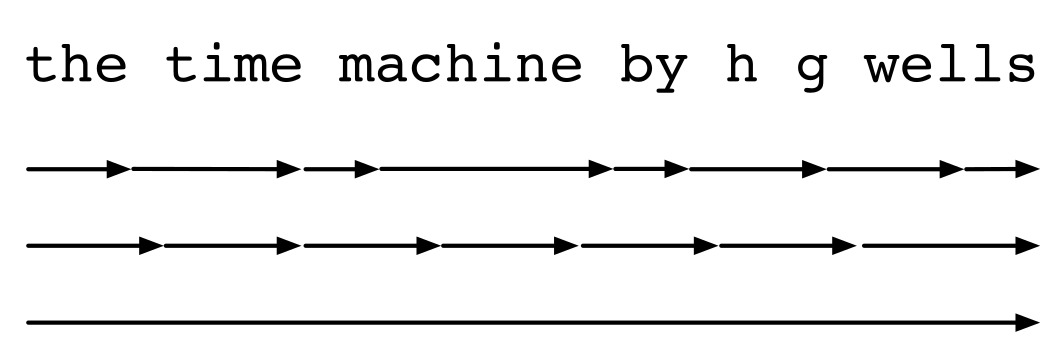
\includegraphics[width=\linewidth, height=1.5cm, keepaspectratio]{Pictures/Recurrent-Neural-Networks/rnn-backprop-strategies.jpg}
    \caption*{From top to bottom: randomized truncation, regular truncation, and full computation}
\end{figure}

\begin{enumerate}
    \item The first row is the randomized truncation that partitions the text into segments of varying lengths.

    \item The second row is the regular truncation that breaks the text into subsequences of the same length. This is what we have been doing in RNN experiments.

    \item The third row is the full backpropagation through time that leads to a computationally infeasible expression.

    \vspace{0.5cm}
    \item while appealing in theory, randomized truncation does not work much better than regular truncation, most likely due to a number of factors. 
    \begin{enumerate}
        \item the effect of an observation after a number of backpropagation steps into the past is quite sufficient to capture dependencies in practice. 
        
        \item the increased variance counteracts the fact that the gradient is more accurate with more steps. 
        
        \item we actually want models that have only a short range of interactions.
    \end{enumerate}
    
    regularly truncated backpropagation through time has a slight regularizing effect that can be desirable.

    
\end{enumerate}


\subsection{Backpropagation Through Time in Detail \cite{dnn-1}}

\begin{customTableWrapper}{1.5}
\begin{longtable}{l l p{8cm}}
    $t$ & $\in \mathbb{R}$ & time step \\
    $T$ & $\in \mathbb{R}$ & number of time steps \\
    $\mathbf{x}_t$ & $\in \mathbb{R}^d$ & single example input \\
    $y_t$ & & target \\

    $\mathbf{W}_\textrm{hx}$ & $\in \mathbb{R}^{h \times d}$ & \\
    
    \hline
    $\phi(x)=x$ & & activation function in the hidden layer uses the identity mapping \\
    $\mathbf{h}_t$ & $\in \mathbb{R}^h$ & hidden state \\
    $\mathbf{W}_\textrm{hh}$ & $\in \mathbb{R}^{h \times h}$ & \\

    \hline
    $\mathbf{o}_t$ & $\in \mathbb{R}^q$ & output \\
    $\mathbf{W}_\textrm{qh}$ & $\in \mathbb{R}^{q \times h}$ & \\

    \hline
    $l(\mathbf{o}_t, y_t)$ & & loss at time step $t$ \\
\end{longtable}
\end{customTableWrapper}

\begin{figure}[H]
    \centering
    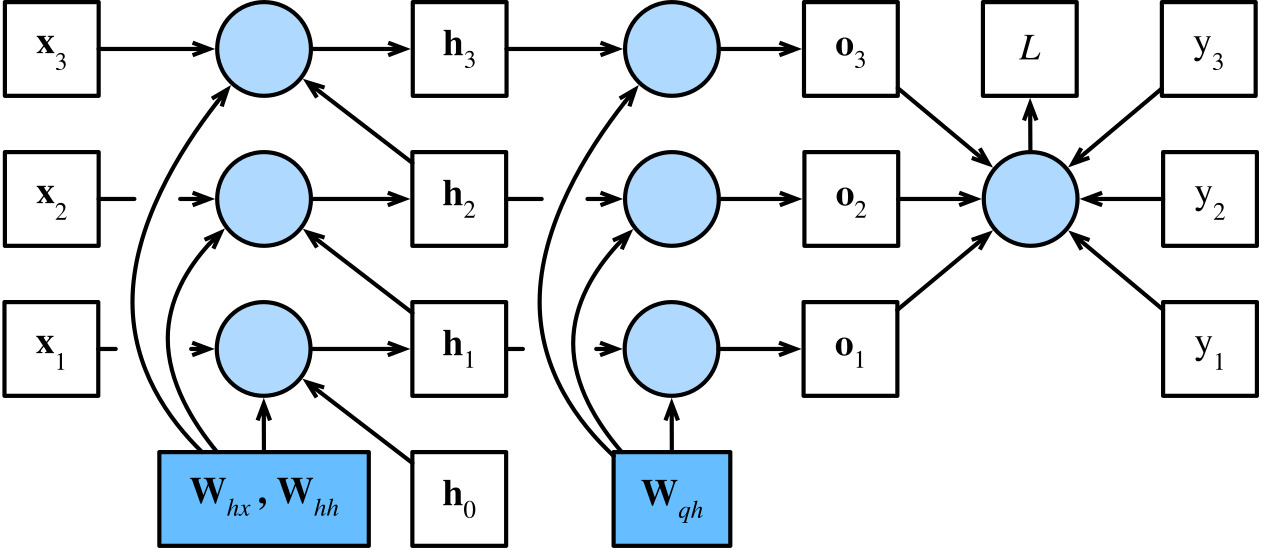
\includegraphics[width=\linewidth, height=3cm, keepaspectratio]{Pictures/Recurrent-Neural-Networks/rnn-bptt.jpg}
    \caption*{Computational graph showing dependencies for an RNN model with three time steps. Boxes represent variables (not shaded) or parameters (shaded) and circles represent operators.}
\end{figure}

\begin{enumerate}[itemsep=0.2cm]
    \item no bias parameters

    \item $
        \hfill
        \mathbf{h}_t = \mathbf{W}_\textrm{hx} \mathbf{x}_t + \mathbf{W}_\textrm{hh} \mathbf{h}_{t-1}
        \hfill
        \mathbf{o}_t = \mathbf{W}_\textrm{qh} \mathbf{h}_{t}
        \hfill
    $

    \item objective function: $L = \dfrac{1}{T} \dsum_{t=1}^T l(\mathbf{o}_t, y_t)$

    \item the computation of the hidden states of time step 3, $h_3$, depends on the model parameters $W_{hx}$ and $W_{hh}$, the hidden state of the last time step $h_2$, and the input of the current time step $x_3$.

    \item According to the dependencies, we can traverse in the opposite direction of the arrows to calculate and store the gradients in turn.\\
    To flexibly express the multiplication of matrices, vectors, and scalars of different shapes in the chain rule.

    \item 
    $
        \dfrac{\partial L}{\partial \mathbf{o}_t} =  \dfrac{\partial l (\mathbf{o}_t, y_t)}{T \cdot \partial \mathbf{o}_t} \in \mathbb{R}^q
        \hfill
    $
    
    \item 
    $
        \dfrac{\partial L}{\partial \mathbf{W}_\textrm{qh}}
        = \dsum_{t=1}^T \left(\dfrac{\partial L}{\partial \mathbf{o}_t} \cdot \dfrac{\partial \mathbf{o}_t}{\partial \mathbf{W}_\textrm{qh}}\right)
        = \dsum_{t=1}^T \dfrac{\partial L}{\partial \mathbf{o}_t} \mathbf{h}_t^\top
        \hfill
        \dfrac{\partial L}{\partial \mathbf{h}_T} = \left(\dfrac{\partial L}{\partial \mathbf{o}_T} \cdot \dfrac{\partial \mathbf{o}_T}{\partial \mathbf{h}_T} \right) = \mathbf{W}_\textrm{qh}^\top \dfrac{\partial L}{\partial \mathbf{o}_T}
        \hfill
    $

    \item 
    $
        \dfrac{\partial L}{\partial \mathbf{h}_t} 
        = \left(\dfrac{\partial L}{\partial \mathbf{h}_{t+1}} \cdot \dfrac{\partial \mathbf{h}_{t+1}}{\partial \mathbf{h}_t} \right) + \left(\dfrac{\partial L}{\partial \mathbf{o}_t} \cdot \dfrac{\partial \mathbf{o}_t}{\partial \mathbf{h}_t} \right) 
        = \mathbf{W}_\textrm{hh}^\top \dfrac{\partial L}{\partial \mathbf{h}_{t+1}} + \mathbf{W}_\textrm{qh}^\top \dfrac{\partial L}{\partial \mathbf{o}_t}
        \hfill
        (t < T)
    $

    \item 
    $
        \dfrac{\partial L}{\partial \mathbf{h}_t}
        = \dsum_{i=t}^T {\left(\mathbf{W}_\textrm{hh}^\top\right)}^{T-i} \mathbf{W}_\textrm{qh}^\top \dfrac{\partial L}{\partial \mathbf{o}_{T+t-i}}
        \hfill
        (1 \leq t \leq T)
    $

    \item 
    $
        \dfrac{\partial L}{\partial \mathbf{W}_\textrm{hx}}
        = \dsum_{t=1}^T \left(\dfrac{\partial L}{\partial \mathbf{h}_t} \cdot \dfrac{\partial \mathbf{h}_t}{\partial \mathbf{W}_\textrm{hx}}\right)
        = \dsum_{t=1}^T \dfrac{\partial L}{\partial \mathbf{h}_t} \mathbf{x}_t^\top
        \hfill
        \dfrac{\partial L}{\partial \mathbf{W}_\textrm{hh}}
        = \dsum_{t=1}^T \left(\dfrac{\partial L}{\partial \mathbf{h}_t} \cdot \dfrac{\partial \mathbf{h}_t}{\partial \mathbf{W}_\textrm{hh}}\right)
        = \dsum_{t=1}^T \dfrac{\partial L}{\partial \mathbf{h}_t} \mathbf{h}_{t-1}^\top
        \hfill
    $

    
\end{enumerate}

















